% !TEX encoding = UTF-8 Unicode
\documentclass[a4paper]{article}

\usepackage{color}
\usepackage{url}
\usepackage[T2A]{fontenc} % enable Cyrillic fonts
\usepackage[utf8]{inputenc} % make weird characters work
\usepackage{graphicx}
\usepackage{parcolumns}
\usepackage[english,serbian]{babel}

\usepackage[unicode]{hyperref}
\hypersetup{colorlinks,citecolor=green,filecolor=green,linkcolor=blue,urlcolor=blue}

\usepackage{lipsum}
\usepackage{listings}
\usepackage{blindtext}
\newtheorem{primer}{Primer}[section]

\definecolor{mygreen}{rgb}{0,0.6,0}
\definecolor{mygray}{rgb}{0.5,0.5,0.5}
\definecolor{mymauve}{rgb}{0.58,0,0.82}

\lstset{ 
  backgroundcolor=\color{white},  
  basicstyle=\scriptsize\ttfamily,        
  breakatwhitespace=false,         
  breaklines=true,                 
  captionpos=b,                    
  commentstyle=\color{mygreen},    
  deletekeywords={...},            
  escapeinside={\%*}{*)},         
  extendedchars=true,              % lets you use non-ASCII characters; for 8-bits encodings only, does not work with UTF-8
  firstnumber=1,                % start line enumeration with line 1
  frame=single,	                   % adds a frame around the code
  keepspaces=true,                 % keeps spaces in text, useful for keeping indentation of code (possibly needs columns=flexible)
  keywordstyle=\color{blue},       % keyword style
  language=PHP,                 % the language of the code
  morekeywords={*,...},            % if you want to add more keywords to the set
  numbers=left,                    % where to put the line-numbers; possible values are (none, left, right)
  numbersep=5pt,                   % how far the line-numbers are from the code
  numberstyle=\tiny\color{mygray}, % the style that is used for the line-numbers
  rulecolor=\color{black},         % if not set, the frame-color may be changed on line-breaks within not-black text (e.g. comments (green here))
  showspaces=false,                % show spaces everywhere adding particular underscores; it overrides 'showstringspaces'
  showstringspaces=false,          % underline spaces within strings only
  showtabs=false,                  % show tabs within strings adding particular underscores
  stepnumber=2,                    % the step between two line-numbers. If it's 1, each line will be numbered
  stringstyle=\color{mymauve},     % string literal style
  tabsize=2,	                   % sets default tabsize to 2 spaces
  title=\lstname                   % show the filename of files included with \lstinputlisting; also try caption instead of title
}

\begin{document}

\title{Programski jezik PHP\\ \small{Seminarski rad u okviru kursa\\Metodologija stručnog i naučnog rada\\ Matematički fakultet}}

\author{Đorđe Vučković, Tamara Ivanović,\\ Petar Simić, Stefan Stevović\\ djordjevuckovic996@gmail.com, tamara.d.ivanovic@gmail.com,\\ petar\_ 95@yahoo.com, stefanstevovic@yahoo.com}

%\date{9.~april 2015.}

\maketitle

\abstract{
U ovom radu su ukratko predstavljene osnovne osobine i specifičnosti programskog jezika PHP. Ovde se možete informisati o razvojnom putu samog jezika, njegovim mogućnostima i primenama.Možete saznati koja su najpoznatija okruženja za programski jezik PHP kao i kako obaviti proces instalacije na Linux i Windows operativnim sistemima. Sam izgled PHP k\^{o}da je prikazan kroz primere koji prate ovaj rad.


\tableofcontents

\newpage

\section{Uvod}
\label{sec:uvod}

\textbf{PHP (Hypertext preprocessor)} je popularan skriptni jezik opšte namene. Nastao je iz potrebe njegovog stvaraoca za praćenjem poseta svog vebsajta i tokom godina sve je popularniji kod veb programera\cite{php}. Kako semantika ovog jezika nije striktna, lak je za učenje, što ga čini pristupačnim programerima sa različitim nivoom znanja \cite{PHPCookbook}.

O popularnosti jezika govore podaci analize GitHub repozitorijuma i projekata. Tokom godina ostaje u prvih 6 jezika po upotrebi. Statistika za period 2012-2014. godine je prikazana u tabeli \ref{tab:tabela1}. Ispred PHP-a 2014. godine su bili jezici JavaScript, Java, Python i CSS\cite{gitinfo}.

Ovaj rad je namenjen svima koji žele da saznaju osnovne karakteristike PHP-a, šta je ono što ga izdvaja od ostalih, kao i kako da ga pokrenu na svojim računarima. Veliki broj radnih okruženja (eng. framework)\cite{learningPHP} je podržan, ali ovde je fokus stavljen na najpoznatija. Ovaj rad se ne fokusira na sintaksu i nema za cilj da čitaoca nauči kako da programira u PHP-u, ali za to preporučujemo knjige ,,Learning PHP", ,,PHP Cookbook" i ,,Programming PHP" \cite{learningPHP, PHPCookbook, programmingPHP}.

\begin{table}[h!]
\begin{center}
\caption{Učešće PHP projekata na GitHub-u i pozicija PHP-a na listi zastupljenosti, u periodu 2012. - 2014. god.}
\begin{tabular}{|c|c|c|c|} \hline
period& PHP repozitorijumi& \% zastupljenosti& pozicija\\ \hline
2012, II kvartal &62336 &11.3 &4\\ \hline
2012, IV kvartal &62336 &8.1 &4\\ \hline
2013, II kvartal &83169 &7.6 &5\\ \hline
2013, IV kvartal &91879 &7.1 &6\\ \hline
2014, II kvartal &118272 &5.6 &6\\ \hline
2014, IV kvartal &138771 &6.3 &5\\ \hline
\end{tabular}
\label{tab:tabela1}
\end{center}
\end{table}

%prošireni podaci tabele, ali zbog izgleda tabele je skraćena
%\begin{tabular}{|c|c|c|c|c|} \hline
%period& broj repozitorijuma& PHP repozitorijumi& \% zastupljenosti& pozicija\\ \hline
%2012, II kvartal &550000 &62336 &11.3 &4\\ \hline
%2012, IV kvartal &770000 &62336 &8.1 &4\\ \hline
%2013, II kvartal &1100000 &83169 &7.6 &5\\ \hline
%2013, IV kvartal &1300000 &91879 &7.1 &6\\ \hline
%2014, II kvartal &1800000 &118272 &5.6 &6\\ \hline
%2014, IV kvartal &2200000 &138771 &6.3 &5\\ \hline



\section{Razvoj programskog jezika PHP}
\textbf{Rasmus Lerdorf} je 1994. godine napravio programski jezik PHP\cite{php}, međutim danas se on značajno razlikuje od početne verzije. Za potrebe napretka svog privatnog vebsajta i praćenja broja poseta, napisao je niz skriptova u C-u koji je nazvao ,,Personal Home Page Tools" , poznatije kao "\textbf{PHP Tools}". Zatim je dodao i mogućnost pristupa bazama podataka kao i kreiranje jednostavnih veb aplikacija. Sledeće godine je PHP Tools bio javno dostupan, mnogi programeri su pomogli da se uklone bagovi i da sam alat napreduje. U septembru iste godine je izbačeno PHP iz imena i alat je dobio naziv \textbf{FI}(eng. Forms Interpreter). Promenljive i sintaksa su bile slične programskom jeziku Perl, za ugnježdavanje koda u HTML fajl bilo je potrebno koristiti HTML komentare. Daljim razvojem i kompletnom izmenom k\^{o}da 1996. godine Lerdorf je objavio \textbf{PHP/FI} \cite{phpfi} koji je od niza alata evoluirao u programski jezik. Tokom iste godine dobio verziju 2.0.

\textbf{Zeev Suraski} i \textbf{Andi Gutmans} su 1997. godine redizajnirali PHP/FI jezgro i nakon toga počeli da sarađuju sa Lerdorfom na pisanju novog programskog jezika. Preimenovan je u PHP(Hypertext Preprocessor), sa promenjenim značenjem jer više nije bilo ograničenja za privatnu upotrebu. Ovo je predstavljalo verziju 3.0. U PHP 3.0 je bila uključena podrška objektno-orijentisanom programiranju, sintaksa jezika je postala konzistentna, a krajnjim korisnicima je omogućen interfejs za API-je, protokole i višestruke baze podataka. U trenutku svog najvećeg uspeha PHP 3.0 je bio instaliran na približno 10\% veb servera na Internetu\cite{php}.


Andri Gutmans i Zeev Suraski su kreirali “\textbf{Zend Engine}” \cite{zend} čija je uloga bila da popravi performanse kompleksnih aplikacija, kao i modulardnost osnove PHP k\^{o}da. Zend Engine je zadužen za leksičku analizu, sintaksno parsiranje i prevođenje koda u bajtkod. Takođe upravlja memorijom i sadrži sakupljač otpadaka. Manipuliše greškama i izuzecima i zadužen je za upravljanje tipovima i promenljivima. Spoj Zend Engine-a i velikog broja dodatnih karakteristika čine PHP 4.0. Ovu verziju odlikuju značajno poboljšane performanse, podrška HTTP sesijama \cite{httpsession} i još većem broju veb servera. Takođe, dodati su i novi jezički konstrukti.

Verzija 5.0 je izašla 2004. godine, a godinu dana kasnije verzija 7.0. Ove dve verzije su najzastupljenije danas, dok prethodne verzije veoma mali broj sajtova koristi. Ovo se može videti na slici \ref{fig:proc_zastupljenosti} koja prikazuje podatke iz 2019. godine prema podacima \cite{stats}. Takođe, na slici \ref{fig:r_stablo} su prikazani programski jezici koji su imali uticaj na razvoj PHP-a.

\begin{figure}[h!]
\begin{center}
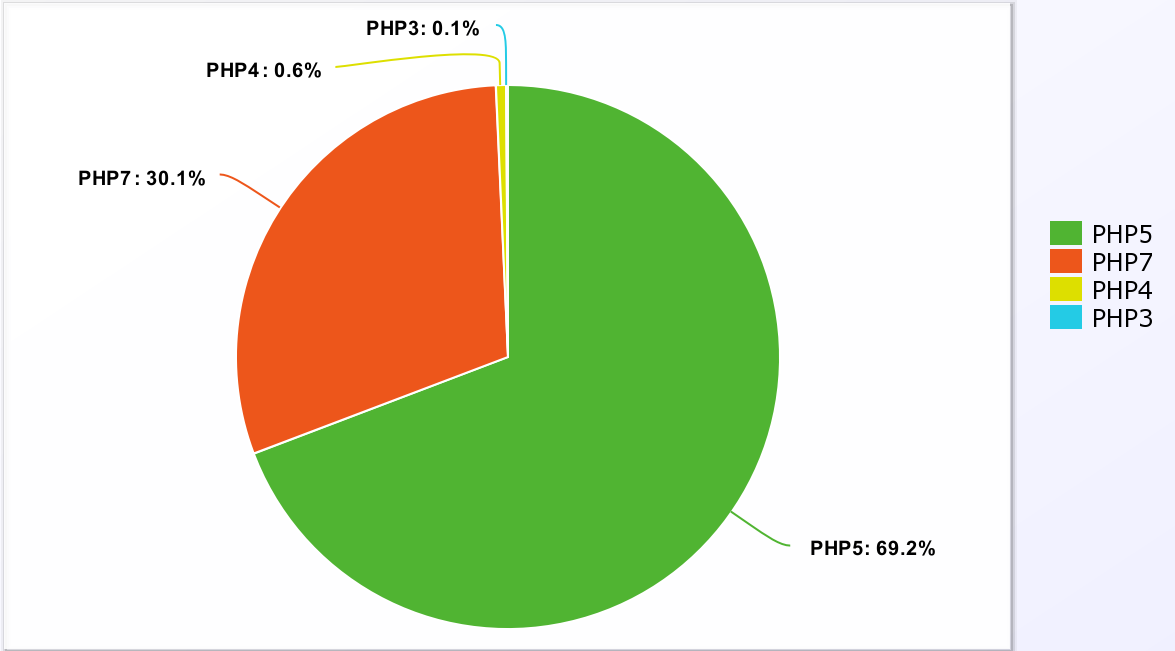
\includegraphics[scale=0.25]{zastupljenost2019.png}
\end{center}
\caption{Procenat sajtova koji koriste određenu verziju PHP-a od ukupnog broja sajtova koji koriste PHP (mart 2019)}
\label{fig:proc_zastupljenosti}
\end{figure}



\begin{figure}[h!]
\begin{center}
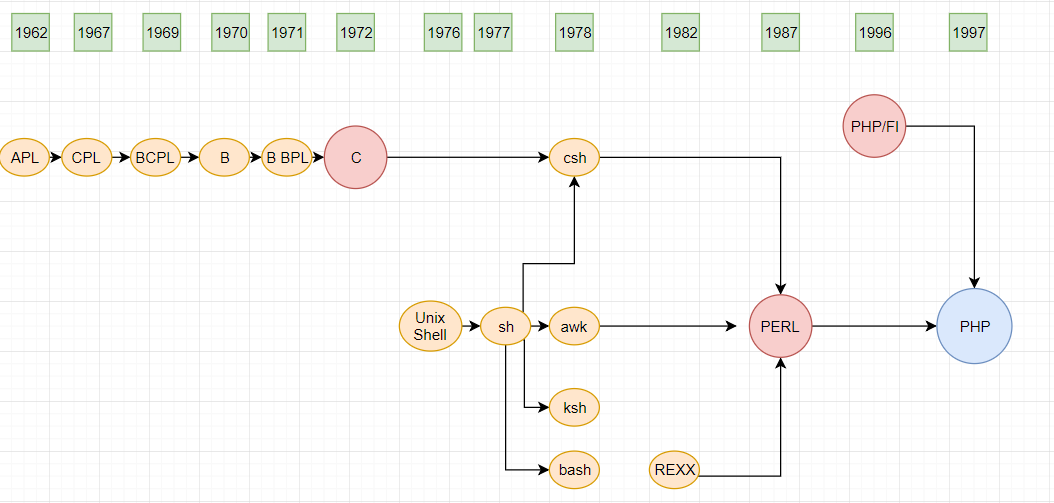
\includegraphics[scale=0.45]{razvojno_stablo.png}
\end{center}
\caption{Razvojno stablo PHP-a}
\label{fig:r_stablo}
\end{figure}

\section{Mogućnosti programskog jezika}
PHP je jezik koji je posebno pogodan za veb razvoj na strani servera, u većini slučaja PHP radi na veb servisu. Može se koristiti na većini veb
servera, mnogim operativnim sistemima i platformama, kao i na mnogim sistemima za upravljanje relacionim bazama podataka (RDBMS). Većina veb hosting provajdera podržaca PHP za upotrebu od strane svojih klijenata. Dostupan je besplatno, a PHP grupa obezbeđuje kompletan izvorni k\^{o}d za korisnike koji će graditi, prilagoditi i proširiti ga za sopstvenu upotrebu. Svaki PHP k\^{o}d u datoteci izvršava PHP runtime\cite{php},
obično da bi kreirao dinamičan sadržaj veb stranica ili dinamičke slike koje se koriste na veb stranicama. Takođe se može koristiti za pisanje
skriptova komandne linije (CLI) kao i za aplikacije grafičkog korisničkog interfejsa na strani klijenta (GUI). Interfejs komandne linije (CLI)
je sredstvo za interakciju sa kompjuterskim programom gde korisni (ili klijent) izdaje naredbe programu u obliku uzastopnih redoba teksta (komandne linije). Programi sa interfejsima komandne linije su uglavnom laki za automatizaciju putem skriptovanja. 

Iako je izvorno dizajniran za korišćenje dinamičkih veb stranicam PHP se sada fokusira uglavnom na pisanje skriptova na strani servera i sličan je drugim skriptnim jezicima na strani servera koji pružaju dinamički sadržaj sa veb servera klijentu. PHP je takođe privukao razvoj mnogih softverskih okvira koji pružaju gradivne blokove i strukturu dizajna za promovisanje brzog razvoja aplikacija (RAD). Brzi razvoj aplikacija je opšti termin koje se koristi za adaptivni pristup razvoju softvera i posebno je pogodan za razvoj softvera koji se pokreće zahtevima korisničkog interfejsa. Neki od njih uključuju PRADO, CakePHP, Simfoni, CodeIgniter, Laravel, Framework, Phalcon i Zend Framework, nudeći mogućnosti slične veb okvirima\cite{PHPtheGoodParts}. Kako dinamičko skriptovanje funkcioniše vidi se na slici \ref{fig:server}. 


\begin{figure}[h!]
\begin{center}
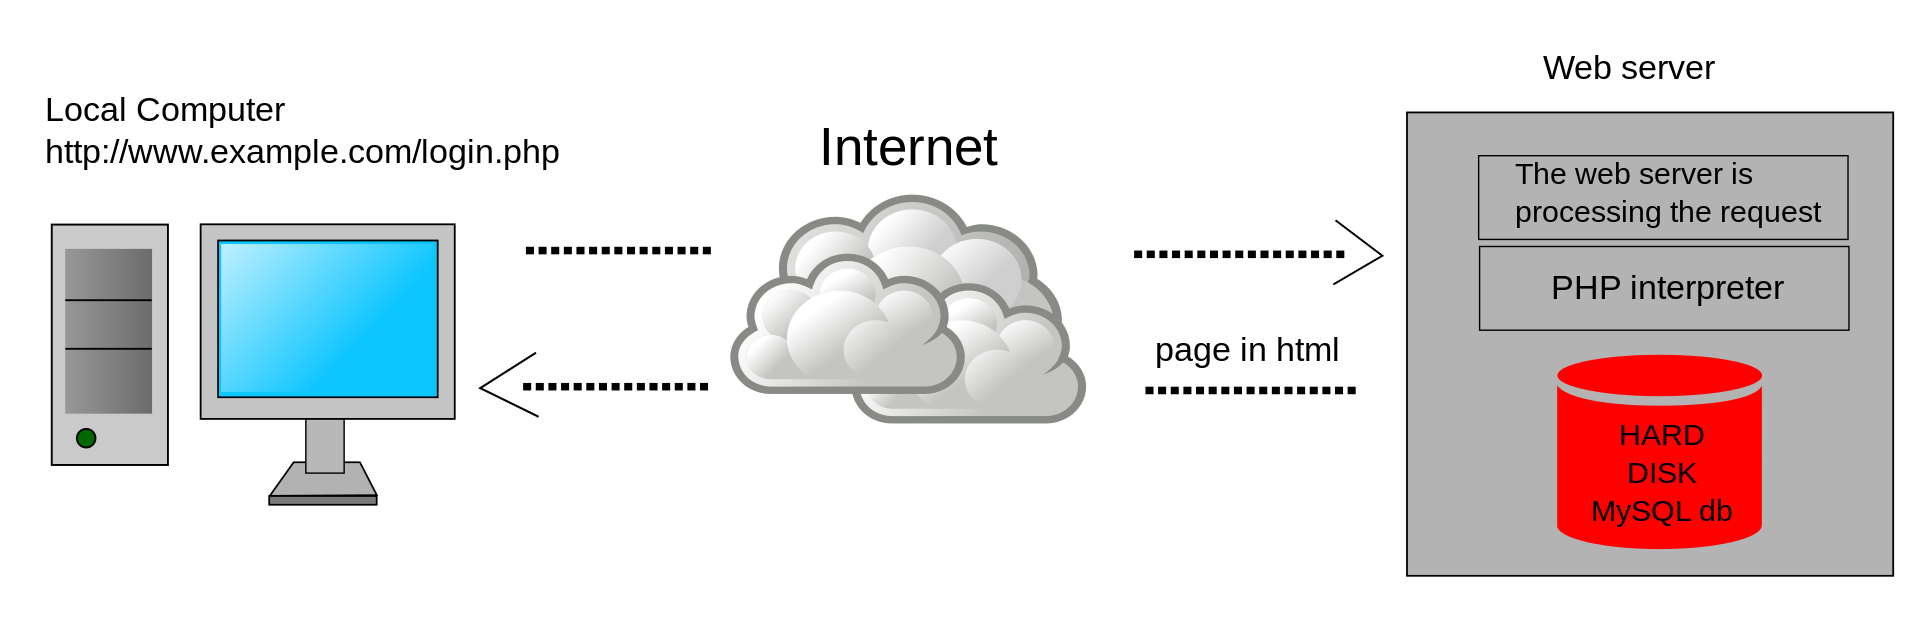
\includegraphics[scale=0.15]{primer_serverskog_skriptiranja.png}
\end{center}
\caption{Dinamička veb stranica: primer serverskog skriptiranja}
\label{fig:server}
\end{figure}
Za specifično i naprednije korišćenje, PHP nudi dobor definisan i dokumentovan način za pisanje prilagođenih ekstenzija u C ili C++ koje dodaju
funkcionalnost jeziku. Ekstenzije se mogu kompajlirati statički u PHP-U ili dinamički učitati tokom izvršavanja. Brojne ekstenzije su napisane kako bi dodale podršku za Windows API i upravljanje procesima na Unix zasnovanim operativnim sistemima. Osim proširivanja samog jezika u obliku dodatnih biblioteka, proširenja pružaju način za poboljšanje brzine izvršavanja tamo gde je ona kritična, a postoji i prostor za poboljšanja korišćenjem kompajliranog jezika. Kompajlirani jezik je programski jezik čija je implementacija obično kompajler (prevodioci koji generišu mašinski kod iz izvornog koda). PHP takođe nudi dobro definisane načine za ugrađivanje u druge softverske projetke. Na taj način se PHP može lako koristiti kao interni skriptni jezik za drugi projekat, a takođe obezbeđuje usko povezivanje sa specifičnim internim strukturama podataka projekta.


\section{Osnovne osobine, podržane paradigme i koncepti}
PHP je sistem koje je svestan interneta i njegovih ugrađenih modula za pristup FTP serverima. Protokol za prenos datoteka (FTP) je mrežni protokol koji služi za prenos datoteka između klijenta i servera na računarskoj mreži. Takođe ima ugrađene module i za pristup raznim serverima baze podataka, uključujući MySQL, Microsoft SKL Server(sistem za upravljanje relacionim bazama podataka koje je razvio Microsoft) i SKLite (koje je ugrađena baza podataka), LDAP (protokol lakog pristupa direktorijumu) servere i druge. 

Neke dodatne PHP karakteristike su dostupne putem proširenja koja uključuju integraciju sa IRC-om (IRC je protokol aplikativnog sloja koji
olakšava komunikaciju u obliku teksta. Proces ćaskanja radi na modelu umrežavanja klijent / server), dinamičku generaciju slika i Adobe Flash sadržaja, PHP Data Objects(PDO je objektno orijentisan interfejs za interakciju sa bazama podataka) kao sloj apstrakcije koji se koristi za pristup bazama podataka, pa čak i sinteze govora. Neke od osnovnih funkicaj jezika, kao što su one koje se bave nizovima, takođe su implementirane kao proširenja\cite{corePHP}.

Drugi projekti, kao što je \textbf{Zephir}\cite{zephir}, pružaju mogućnost da PHP ekstenzije budu kreirane na jeziku visokog nivoa i kompajlirane u izvorne PHP ekstenzije. Takav pristup, umesto pisanja PHP ekstenzija direktno u C, pojednostavljuje razboj ekstentija i skraćuje vreme potrebno za programiranje i testiranje.

Originalna i najraširenija implementacija PHP-a pokreće Zend Engine i poznaza je kao PHP. Da bi se razdvojila od drugih implementacija, ponekad se nezvanično zove ‚‚Zend PHP". PHP-ov model ‚‚\textit{jedan-zahtev-za-skriptom-izvršenje}" i činjenica da je Zend Engine interpreter dovodi do neefikasnosti. Kao rezultat toga, razvijeni su razni proizvodi koji pomažu poboljšanju performansi PHP-a. Kako bi se ubrzalo vreme izvršavanja i da se ne mora kompajlirati PHP izvorni k\^{o}d svaki put kada se pristupi veb stranici, PHP skripte se mogu primeniti u unutrašnjem formatu PHP mašine korišćenjem operacionog keša. Operacioni keš funkcioniše tako što kešira kompajlirani oblik PHP skript u zajedničkoj memoriji kada se skripta pokrene. Jedan od operacionih keševa, Zend Opcache\cite{zend}, je ugrađen u PHP od verzije 5.5. Drugi primer široko korišćenog operacionog keša je alternativni PHP keš (APC je besplatan i otvoren okvir koji kešira izlat PHP kompajlera u zajedničku memoriju)\cite{php}, koji je dostupan kao PECL ekstenzija.

Iako je Zend PHP još uvek najpopularnija implementacija, razvijeno je nekoliko drugih implementacija. Neko od njih su kompajleri ili podržavaju
JIT\cite{jit} kompilaciju i stoga nude prednosti u odnosu na Zend PHP na račun nedostatka potpune PHP kompatibilnosti. Alternativne implementacije uključuju:

\begin{itemize}
\item \textbf{HHVM(HipHop Virtual Machine)}\cite{hhvm} - razvijen na Facebook-u i otvorenog koda, pretvara PHP k\^{o}d u bajt-k\^{o}d visokog nivoa, koji je obično poznat kao posredni jezik, koji se potom pretvara u k86-64 mašinski k\^{o}d. U vremenu izvršavanja kompajler je pravedan u vremenu (JIT), što rezultira poboljšanjem performansi do šest puta.
\item \textbf{Parrot}\cite{parrot} - virtuelna mašina dizajnirana da efikasno pokreće dimaničke jezike. Pipp(mali PHP programski okvir) transformiše PHP izvorni k\^{o}d u Parrot posrednu reprezentaciju, koja se zatim prevodi u Parrot-ov bajt k\^{o}d i virtuelna mašina ga izvršava.
\item \textbf{Phalanger} - sastavlja PHP u bajt k\^{o}d Common Intermediate Language (CIL)
\item \textbf{Kuercus} - kompajlira PHP u java bajt k\^{o}d.
\end{itemize}

Već je rečeno da je PHP skriptni jezik opšte namene. Pored toga on podržava još mnoge koncepte. Od verzije 5.0 ima jaku podršku za \textbf{objektno-orijentisano programiranje}. To uključuje podršku za nasleđivanje, konstruktore, izuzezke, interfekse, klase i apstrakne klase. Takođe, podržava i funkcije prve klase(eng. first-class functions) što znači da funkcija može biti dodeljena promenljivoj. Korisnički definisane funckije, kao i ugrađene funkcije mogu biti referisane od strane promenljive i pozivaju se dinamički. Podržava rekurziju, odnosno da funkcija poziva samu sebe, mada kod PHP-a je fokus na iteraciji. Funkcije se mogu prosleđivati kao argumenti tj. funkcije višeg reda i funkcija može vratiti druge funkcije. Od verzije 5.3 uvedena je i podrška za anonimne funkcije sa podrškom za zatvorenje. Verzija 5.4 je dodala mogućnost povezivanja zatvaranja sa opsegom objekta i poboljšanu podršku za callables tako da se mogu koristiti naizmenično sa anonimnim funkcijama u gotovo svim slučajevima. Ove osobine opravdavaju pripadanje \textbf{funkcionalnoj paradigmi} \cite{phpSrbija}.


\section{Najpoznatija okruženja}
Na samom početku ovog poglavlja treba da se upoznamo sa terminom \textbf{razvojno okruženje} (eng. framework). Razvojno okruženje predstavlja skup već gotovih komponenti koje čine skelet startne platforme. Ta platforma omogućava da se bude brži i efikasniji pri pisanju programa. Najbitniji faktor je to što se povećava brzina programiranja jer se ne počinje svaki put od nule već su na raspolaganju raznorazni gotovi moduli koji se mogu jednostavno koristiti. Razvojno okruženje čini rad na zahtevnim projektima jednostavnijim, omogućava pisanje čistog i ponovo upotrebljivog k\^{o}da i  sugeriše na moguće greške.

Postoje razna razvojna okruženja za svaki programski jezik pa tako i za PHP. Koje razvojno okruženje izabrati zavisi najviše od samog projekta. Za jezik PHP najpoznatija razvojna okruženja su Laravel\cite{laravel}, CodeIgniter\cite{codeigniter} i Symfony\cite{symfony}.

\textbf{Laravel} programeri najviše koriste zbog njegove brzine, fleksibilnog rutiranja i mogućnosti upravljanja preko komandne linije. Odlikuje ga jednostavno i intuitivno korišćenje kao i čist i pregledan k\^{o}d. U potpunosti je baziran na MVC arhitekturi eng(Model Wiew Controller).

\textbf{CodeIgniter} je razvojno okruženje koga odlikuje bezbednost, poseduje zaštitu od XSS i CSRF napada. Uopšte nije memorijski zahtevan jer zauzima svega par megabajta. Omogućava MVC arhitekturu, ali nije striktan po tom pitanju. Poseduje sveobuhvatnu dokumentaciju koja se dobija uz samo razvojno okruženje.

Pored sjajnih osobina poput brzine, fleksibilnosti, ponovno upotrebljivih komponenti, razvojno okruženje \textbf{Symfony} karakteriše izuzetna podrška. Osim podrške koju pruža sama firma Sensio, tvorac ovog razvojnog okruženja, veliki broj profesionalaca i firmi koristi upravo Symfony, pa je samim tim moguće dobiti odgovore na sva pitanja. Ovo razvojno okruženje podržava trenutne standarde PHP-a i pored toga omogućava korisnicima da koriste delove vlastitog softvera, bez da koriste celo razvojno okruženje.

\section{Instalacija}
Za kreiranje interaktivnih veb stranica i izvršavanje PHP programa neophodan je server koji podržava PHP. Prilikom samog razvoja bilo kog PHP projekta komunikacija sa tim serverom je veoma česta, stoga je izuzetno nepraktično stalno komunicirati sa nekim udaljenim serverom. Iz tog razloga se preporučuje instalacija lokalnog servera. Osim servera potrebna je i baza podataka. Naravno osim servera i baze, potrebno je instalirati i sam jezik PHP. Na novijim operativnim sistemima PHP uglavnom dolazi uz sam sistem, ali će ovde instalacija biti objašnjena od samog početka, kao da ništa od potrebnog nije instalirano.

Dakle, potrebni su sam PHP programski jezik, server i baza podataka. Postoji mogućnost da se zasebno svaka od navedenih stavki instalira i podešava, ali postoji i mnogo lakši način, a to su LAMP(linux apache mySql PHP) \cite{lamp} i WAMP(windows apache mySql PHP) \cite{wamp} serveri. 

Na operativnom sistemu \textbf{Windows} sama instalacija se sastoji od preuzimanja WAMP servera sa stranice:\url{http://www.wampserver.com/en/} , zatim sledi pokretanje preuzetog fajla koje automatski pokreće instalaciju celog paketa. Sam proces nadalje je automatizovan i WAMP server paket stiže sa najnovijim verzijama Apache-a, MySQL-a i PHP-a. Nakon procesa instalacije biće kreirana prečica ka WampServer-u kao i  folder www, obično na putanji c:\textbackslash \textbackslash wamp\textbackslash \textbackslash www. Nakon toga u folderu www potrebno je kreirati poddirektorijum koji će služiti za smeštanje PHP fajlova. Na primer, kreiran je fajl 1.php. Moguće je otvoriti ga u veb pregledaču, tako što se u meniju WampServer-a klikne na link “localhost” ili se u pregledaču ukuca http://localhost/1.php.

Kod operativnog sistema \textbf{Linux} instalacija se vrši preko terminala i zahteva instaliranje svake komponente pojedinačno, što je prikazano u \ref{instalacija}. 

\begin{lstlisting}[language=bash, caption={Pokretanje instalacije na Linux operativnom sistemu}, label={instalacija}]
sudo apt-get update #update sistema
sudo apt-get install apache2 #instalacija Apache-a
sudo apt-get install mysql-server libapache2-mod-auth-mysql php5-mysql #instalacija MySQL-a
sudo mysql_install_db #instalacija MySQL servera
sudo /usr/bin/mysql_secure_installation #pokretanje skripte za podesavanje MySQL-a
sudo apt-get install php5 libapache2-mod-php5 php5-mcrypt #instalacija PHP-a

\end{lstlisting}
Po završetku instalacije MySQL-a može biti traženo da se postavi root šifra što je i potrebno uraditi.

PHP takođe sadrži veliki broj korisnih biblioteka i modula koji se mogu dodati na  server. Za izlistavanje potrebno je pokrenuti komandu “apt-cache search php5-” i biće prikazani svi moduli. Za instalaciju nekog od tih modula služi komanda “sudo apt-get install <ime\_ modula>”. Nakon što je instaliran LAMP može se pokrenuti prethodno napravljeni program, npr. 1.php. Potrebno je smestiti ga u /var/www direktorijum i može se pokrenuti preko pregledača ukoliko se ukuca http://localhost/1.php. 

\section{Primer k\^{o}da}
\begin{primer}
Primer kako se pomoću PHP-a može konektovati na bazu podataka, izvršiti upit i ispitati dobijene rezultate. Cilj u ovom primeru \ref{primer_koda} je pronaći sve studente sa zadatim imenom i prezimenom i ispitati njihov datum rođenja.
\end{primer}


\begin{lstlisting}[caption={Primer PHP k\^{o}da},frame=single, label=primer_koda]
<?php
	//uspostavljanje konekcije sa bazom podataka
	if(mysqli_connect_errno()){
		die("Problem sa povezivanjem: ".mysqli_connect_error());
	}
	//deklarisanje promenljivih i ucitavanje podataka
	$ime = $_GET['ime'];
	$prezime = $_GET['prezime'];
	//formulisanje i izvrsavanje upita
	$upit = " select datum_rodjenja from dosije where ime = '$ime' and prezime = '$prezime' ";
	//rezultat upita se smesta u promenljivu rezultat
	$rezultat = mysqli_query($veza, $upit) or die("Problem prilikom izvrsavanja upita: ".mysqli_error($veza));
	
	//racunanje broja redova rezultata (broj studenata sa zadatim imenom i prezimenom)
	$broj_pojavljivanja = mysqli_num_rows($rezultat);
	if($broj_pojavljivanja == 0){
		echo "Nema studenata koji se zovu $ime $prezime.";	
	}
	else{
		//ukoliko ima studenata ispisujemo ih	
		echo "<ul>";
		for($i=0; $i<$broj_pojavljivanja; $i++){
			$red = mysqli_fetch_assoc($rezultat);
			echo "<li>";
			echo $red['ime']['prezime']['datum_rodjenja'];
			echo "</li>";		
		}
		echo "</ul>";
	}
	//raskidamo konekciju sa serverom
	mysqli_close($veza);
?>
\end{lstlisting}
Sav PHP k\^{o}d se piše između “<?php“ i “?>“, slično kao tagovi pri pisanju html k\^{o}da. Promenljive deklarišemo sa prefiksom “\$“ a naredbom “echo“ vršimo ispis. \$\_ GET metod smo koristili kako bismo preneli vrednosti promenljivih kroz veb stranicu do našeg k\^{o}da. Vrednosti tih promenljivih se dodaju u URL stranicu. Na primer ako bismo želeli da izlistamo sve studente koji se zovu Marko i prezivaju Marković, to bismo uradili tako što bismo u URL adresu dodali ?ime=Marko\& prezime=Markovic.

\section{Specifičnosti}

Ono što je veoma specifično za ovaj jezik jeste to što nema striktnu sintaksu koja prati veliki broj jezika. Na primer, sledeći fragment k\^{o}da možemo zapisati na dva razlicita načina. Kao što je prikazano u \ref{fig:stand_alt} standardni pristup koristi vitičaste zagrade, dok je u alternativnom pristupu fokus na elseif grananju. 

\begin{figure}[h]
		\centering
		\begin{minipage}{0.35\textwidth}
\begin{lstlisting}
<?php
if($a > 0){
	echo "a ima pozitivnu vrednost";
} elseif($a == 0){
	echo "a je nula";	
} else{
	echo "a ima negativnu vrednost";	
}
?>	
\end{lstlisting}
		\end{minipage}
		\hfill
		\begin{minipage}{0.35\textwidth}
\begin{lstlisting}
<?php
if($a > 0):
	echo "a ima pozitivnu vrednost";
elseif($a == 0):
	echo "a je nula";	
else:
	echo "a ima negativnu vrednost";	
endif;
?>	
\end{lstlisting}
		\end{minipage}
		\caption{Primer dva fragmenta koda standardni pristup (levo) i alternativni pristup (desno).}
		\label{fig:stand_alt}
\end{figure}



\textbf{Imenski prostor} (eng. namespace) \cite{phpSrbija} je uveden od verzije 5.3 i prevashodno je zamišljen radi rešavanja konflikata oko istoimenih metoda i funkcija, kako bi mogle da se koriste u okviru istog projekta. Ovo je posebno pogodno u slučaju da se radi o kompleksnim projektima, koji su raspoređeni po različitim datotekama i kada u razvoju aplikacije učestvuje grupa programera. Za deklarisanje imenskog prostora koristi se ključna reč \textbf{namespace}. Dozvoljeno je koristiti više imenskih prostora u okviru istog programa, čak i iste datoteke.

Još jedan veoma bitan koncept u radu sa PHP programima jeste rad sa formama. Forma je zapravo deo HTML strukture za grupisanje različitih elemenata čija je funkcija prikupljanje podataka od korisnika. U zavisnosti od akcije korisnika, dobijena informacija se može proveriti kod korisnika. Takođe se može proslediti kao zahtev serveru, eventualno na ponovnu proveru i kasniju obradu. Po potrebi na kraju se može poslati neka vrsta povratne informacije korisniku. Forme se koriste, na primer, kod poručivanja hrane u piceriji preko interneta. Popunjavamo formular gde biramo vrstu pice, dodatke, adresu gde će se pica dostaviti itd. Nakon obrade i čitanja podatka iz forme, šalje se odgovor da je porudžbina primljena i da će pica ubrzo stići.

Jezik PHP se odlikuje ogromnim brojem različitih klasa koje u mnogome olakšavaju rad programerima. Jedna veoma bitna klasa je “PDO (PHP Data Object)”\cite{PHPtheGoodParts, phpSrbija} koja se koristi za povezivanje sa SQL bazama podataka. Ta klasa obezbeđuje sloj apstrakcije za skup upravljačkih programa za baze podataka kao što su MySQL, PostgreSQL i MSSQL. To znači da ma koju bazu podataka koristili, ako je PDO podržava, možemo koristiti iste funkcije za izvršavanje istih operacija nad bazom podataka. To čini k\^{o}d i samu aplikaciju portabilnom u smislu da se može koristiti u različitim bazama podataka bez nekakve modifikacije samog k\^{o}da.

Još jedna veoma korisna i zamiljiva klasa je DateTime klasa \cite{PHPtheGoodParts, phpSrbija} koja služi za reprezentaciju vremena i datuma. Pored jednostavnog definisanja i ispisa trenutnog vremena koje je predstavljeno u \ref{datum}, ova klasa sadrži ogroman broj različitih funkcija za rad sa datumima poput izdvajanja dana, meseca, godine iz datuma i postavljanje vremenskih zona. 

\begin{lstlisting}[caption={Primer upotrebe klase DateTime},frame=single, label=datum]
$d = new DateTime('2019-01-01T15:03:01.012345z')
echo $d -> format('Y-m-d\TH:i:s.u') //2019-01-01T15:03:01.012345
\end{lstlisting}

Ono što se u jeziku PHP dosta koristi jesu \textbf{kolačići} (eng. cookies)\cite{PHPtheGoodParts, phpSrbija} koji se često koriste za identifikaciju korisnika. Kolačić je mala datoteka koju server ugrađuje na računar korisnika. Svaki put kada isti računar zahteva stranicu, ona će takođe poslati i kolačić. Pomoću PHP-a možemo kreirati i dohvatiti vrednosti kolačića. Funkcija koja postavlja vrednost kolačića je data u primeru \ref{kolacici}.

\begin{lstlisting}[caption={Funkcija za postavljanje kolacica},frame=single, label=kolacici]
setcookie(name, value, expire); //postavljanje kolacica
setcookie("user", "", time() - 3600); //brisanje kolacicaica
\end{lstlisting}

Pristup disku je spor dok je pristup mreži još sporiji. Baze podataka obično koriste oba. Korišćenje lokalnog keša izbegava opterećenje mreže i pristupa disku. Kombinujući ove pristupe dobijamo sistem za memorisanje objekata distribuirane memorije (eng. memcached) \cite{tips}. Ako naša aplikacija nije distribuirana na više servera, verovatno nam neće trebati memcached. Jednostavniji pristupi keširanju su na primer serijalizovanje podataka i čuvanje u privremenoj datoteci, na primer - mogu eliminisati mnogo redundantnih podataka na svakom pojedinačnom zahtevu\cite{phpSrbija}. Primer keširanja je dat primerom \ref{kesiranje}.

\begin{lstlisting}[caption={Primer keširanja},frame=single, label=kesiranje]
<?php
$feed = apc_fetch('news');
if ($feed === FALSE) {
    $feed = file_get_contents('http://example.org/news.xml');
    // Cuvanje podataka u deljenoj memoriji 5 minuta (5*60 sekundi)
    apc_store('news', $feed, 300);
}
// Uradi nesto sa $feed.
?> 
\end{lstlisting}




\section{Zaključak}
\label{sec:zakljucak}

Programski jezik PHP značajno olakšava veb programiranje i zbog toga je među jednim od najpopularnijih programskih jezika današnjice. Pored toga, rad sa bazama podataka je dosta jednostavan, pa to predstavlja jednu od najbitnijih olakšica u veb programiranju, korišćenjem PHP-a. Mogućnosti ovog jezika su velike, međutim kroz ovaj rad su predstavljene samo one koje ga ističu u odnosu na druge. Takođe, ovim radom smo istakli sve ono što bi programere koji se do sad nisu susreli sa  PHP-om zainteresovalo da počnu da ga koriste.


\addcontentsline{toc}{section}{Literatura}
\appendix
\bibliography{seminarski} 
\bibliographystyle{plain}



\end{document}
